% !TEX enableShellEscape = true

\documentclass[10pt]{article}
\usepackage[cache=false]{minted}
\usepackage{fullpage}
\usepackage{graphicx}

\author{Johnathan DiMatteo}
\title{CS 885: Reinforcement Learning Assignment 2}
\date{June 29th 2018}

\begin{document}
\graphicspath{{./Images/}}
\maketitle
\pagebreak
\tableofcontents
\pagebreak

\section{Question 1}

\paragraph{Bandit #1: Epsilon Greedy}
done

\paragraph{Bandit #2: Thompson Sampling}
done

\paragraph{Bandit #3: UCB}
done

%%
\begin{table}[!th]
  \begin{tabular}{|c|c|}
    \hline
    Number of Iterations in Partial Evaluation (i) & Number of Iterations Total\\ \hline
    1 & 8 \\
    2 & 7 \\
    3 & 6 \\
    4 & 6 \\
    5 & 5 \\
    6 & 5 \\
    7 & 5 \\
    8 & 5 \\
    9 & 5 \\
    10 & 5 \\
    \hline
  \end{tabular}
  \centering
  \caption{Varying the number of iterations for Partial Policy Evaluation}
  \label{mdp}
  \centering
\end{table}


\ref{mdp} shows how at i = 5 the modified policy iteration algorithm converges with the same number of
total iterations as the policy iteration algorithm, and no improvement is seen past this. Since
Modified Policy Iteration follows a linear-quadratic convergence \\
$O(i \times |S^2| + |S^2| \times |A|)$, as long as $i \leq |A|$, it is cheaper
to evaluate.

\section{Model-Based RL}
implementing Q function


\section{REINFORCE}
not completed

\section{}

\section{Question 2}
% chart
\begin{figure}[h]
  \caption{Cumulative Rewards vs Episode}
  \label{q2}
  \centering
  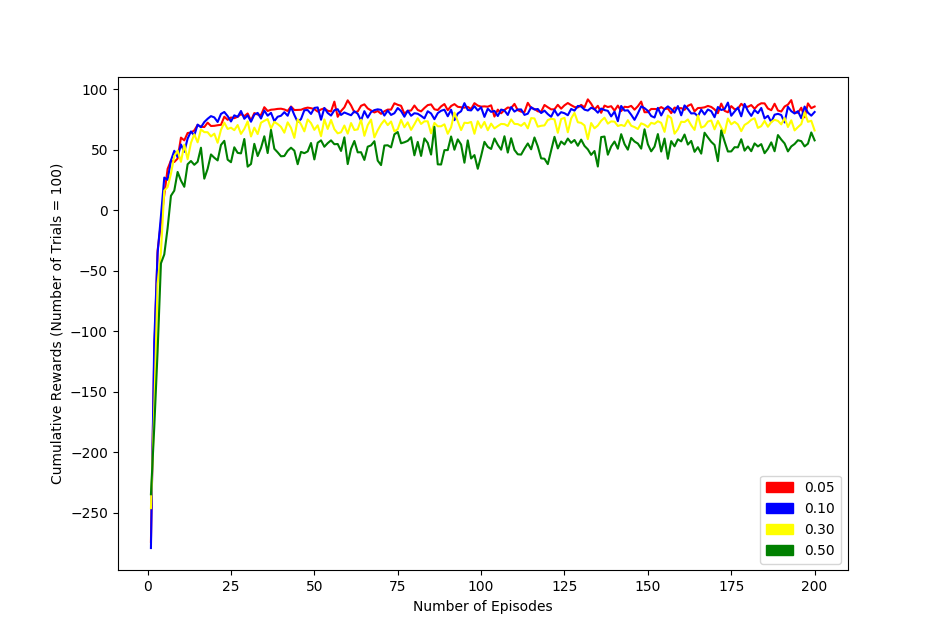
\includegraphics[width=\textwidth]{q2}
\end{figure}



\inputminted{python}{RL2.py}

\end{document}
